\documentclass[conference]{IEEEtran}
\IEEEoverridecommandlockouts
% The preceding line is only needed to identify funding in the first footnote. If that is unneeded, please comment it out.
\usepackage{cite}
\usepackage{amsmath,amssymb,amsfonts}
\usepackage{algorithmic}
\usepackage{textcomp}
\usepackage{xcolor}
\usepackage{colortbl}
\usepackage[rightcaption]{sidecap}
\usepackage{wrapfig}
\usepackage{adjustbox}
\usepackage{siunitx}
\usepackage{hyperref}
\def\UrlBreaks{\do\/\do-}
\usepackage{graphicx} %package to manage images
\graphicspath{ {./images/} }


\def\BibTeX{{\rm B\kern-.05em{\sc i\kern-.025em b}\kern-.08em
    T\kern-.1667em\lower.7ex\hbox{E}\kern-.125emX}}
\begin{document}

\title{Online Store Application: Art Store+}

\author{\IEEEauthorblockN{1\textsuperscript{st} Tomás Marcos}
\IEEEauthorblockA{\textit{Faculdade de Ciências Exatas e da Engenharia} \\
\textit{Universidade da Madeira}\\
Funchal, Portugal \\
2037017@student.uma.pt}
\and
\IEEEauthorblockN{2\textsuperscript{nd} Nelson Vieira}
\IEEEauthorblockA{\textit{Faculdade de Ciências Exatas e da Engenharia} \\
\textit{Universidade da Madeira}\\
Funchal, Portugal \\
2080511@student.uma.pt}
\and
\IEEEauthorblockN{3\textsuperscript{rd} Luís Olim}
\IEEEauthorblockA{\textit{Faculdade de Ciências Exatas e da Engenharia} \\
\textit{Universidade da Madeira}\\
Funchal, Portugal \\
2034717@student.uma.pt}
}

\maketitle

\begin{abstract}
 \\
\end{abstract}

\begin{IEEEkeywords}

\end{IEEEkeywords}

\section{Introdução}

\IEEEPARstart{A}rte, do latin ars que significa técnica e/ou habilidade, pode ser entendida 
como a atividade humana ligada às manifestações de ordem estética ou comunicativa, realizada 
por meio de uma grande variedade de linguagens, tais como: arquitetura, desenho, escultura, 
pintura, escrita, música, dança, teatro e cinema, em suas variadas combinações. \cite{wikiarte}

`Desde sempre a arte funcionou como espelho da sociedade, 
acompanhando cada contemporaneidade ao longo dos tempos, deixando registado na sua obra os diferentes 
momentos vividos, com intensidade e questionamento, como um diário pessoal da humanidade, 
desde que o Homem se pensou como tal.` \cite{patrimonio}



\subsection{Formas de arte}
As artes são, muitas vezes, divididas em categorias específicas, tais como artes decorativas, 
artes plásticas ou visuais, artes do espectáculo, ou literatura.

\subsection{Objetivos}

\section{Métodos e Metadologias}

O trabalho descrito neste artigo pretende 

\subsection{Tecnologias utilizadas}

A aplicação que propomos, é uma aplicação que foi desenvolvida utilizando:

\begin{itemize}
    \item Figma - software de prototipagem;
    \item FlutterFlow - aplicação web para desenvolvimento de aplicações à base de Flutter;
    \item Flutter - linguagem para desenvolvimento de aplicações móveis;
    \item Firebase - plataforma para desenvolvimento de aplicações, atualmente pertencente à Google;
    \item Firestore - base de dados do Firebase;
    \item VSCode - IDE utilizado para escrita do código;
    \item Git - plataforma de controlo de versões;
\end{itemize}

Primeiramente, foram realizados alguns esboços sobre qual poderia ser a aparência da aplicação. A figura \ref{fig:sketches} 
mostra os esboços realizados para a aplicação.

\begin{figure}[h]
    \centering
    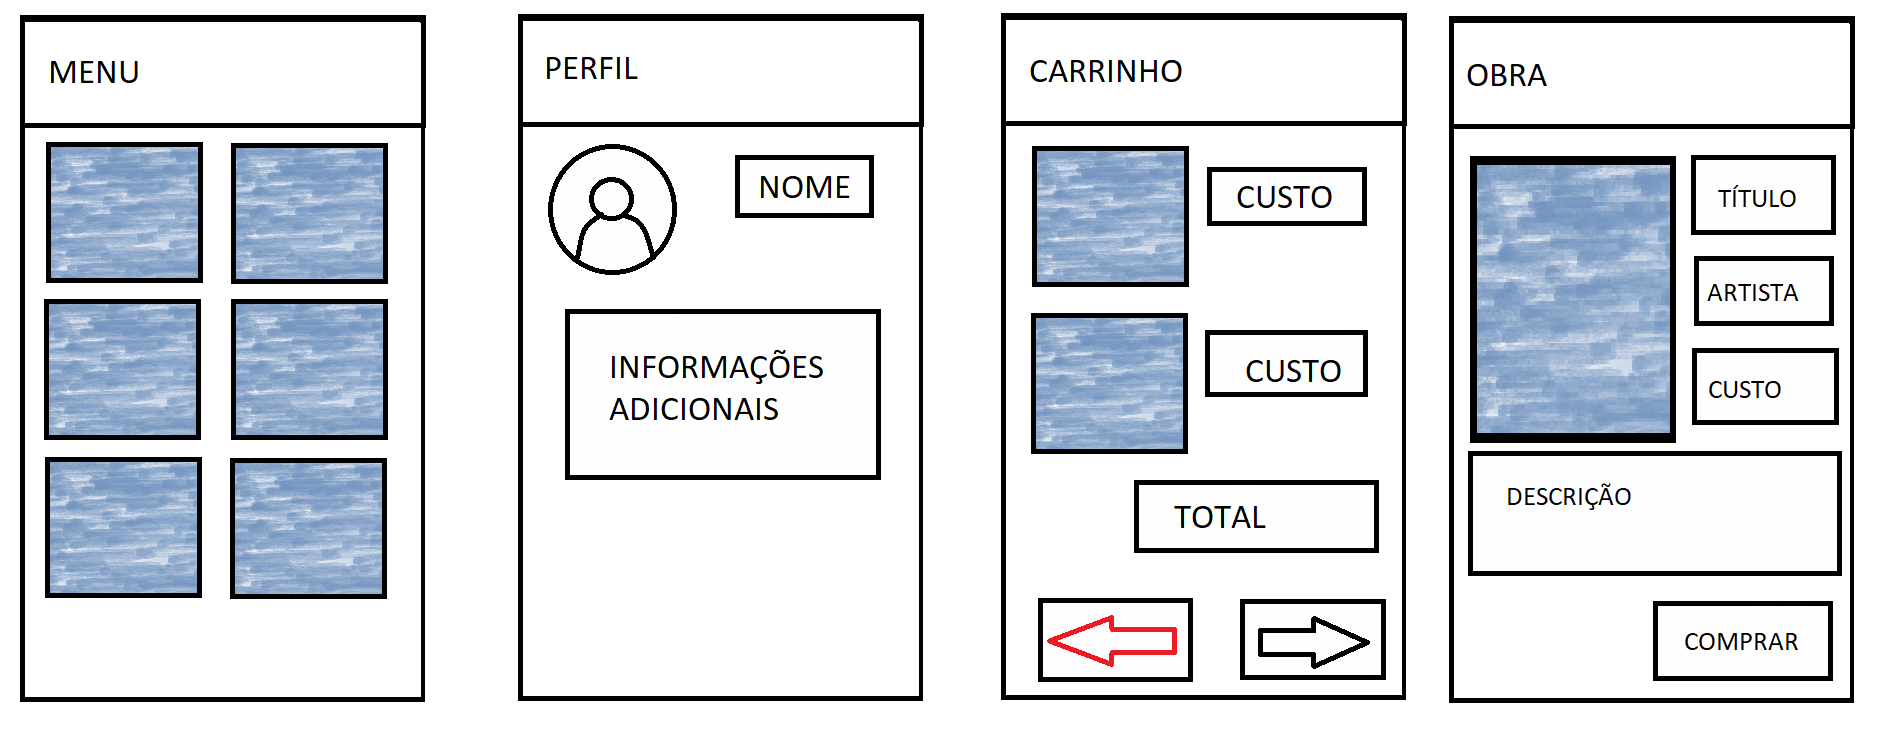
\includegraphics[width=0.5\textwidth]{appsketches.png}
    \caption{Esboços da aplicação}
    \label{fig:sketches}
\end{figure}

A partir dos esboços criados, procedeu-se à realização de um protótipo no Figma, de maior fidelidade, tal que 
fosse possível testar algumas funcionalidades da aplicação.

\subsection{Testes}

\subsection{Problemas Encontrados}

Durante a realização do projeto descrito neste artigo, surgiram vários problemas, 

\section{Conclusão e Trabalho Futuro}

\bibliographystyle{IEEEtran}
\bibliography{references}

\end{document}


